An implicit $r$-step LMM of the form

$$U^{n+r}=U^{n+r-2}+h\sum_{j=0}^r\beta_jf(t_{n+j},U^{n+j}),\;\;\;\beta_r\neq0$$

is known as the implicit Milne Method.\\
a. Derive the 2-step third order accurate Milne Method, starting from the relation

$$u(t_{n+2})=u(t_n)+\int_{t_n}^{t_{n+2}}f(s,u(s))ds$$

and following the procedure described in exercise 5.10.b. in LeVeque.\\
b. Use the implicit Milne's method to solve numerically the ODE

$$u'(t)=2(t+1),\;\;\;u(1)=3$$

\begin{solution}\renewcommand{\qedsymbol}{}\ \\
    a. From the prcedure in LeVeque, we will continue with Newton's Method for the derivation. Since it
    is recommended that we approximate up to a quadratic, indeed since this is a two step this makes
    sense, that is precisely what we will do. First note that will we have a quadratic equation of the
    from $p(t)=A+B(t+h)+C(t+h)t$. By Newton's method, we have that

    $$A=f(U^n)\;\;B=\frac{f(U^{n+1})-f(U^n)}{t_{n+1}-t_n}$$
    $$C=\frac{\frac{f(U^{n+2})-f(U^{n+1})}{t_{n+2}-t_{n+1}}-\frac{f(U^{n+1})-f(U^n)}{t_{n+1}-t_n}}
    {t_{n+2}-t_n}$$

    Since we are considering uniform time steps, we have that $t_{n+2}-t_{n+1}=t_{n+1}-t_n=h$ and that
    $t_{n+2}-t_n=2h$. Hence, $B=\frac{f(U^{n+1})-f(U^n)}{h}$ and
    $C=\frac{f(U^{n+2})-2f(U^{n+1})+f(U^n)}{2h^2}$. So, integrating $p(t)$ from $t_n=-h$ to $t_{n+2}=h$
    yields

    $$\int_{t_n}^{t_{n+2}}p(t)d$$
    $$=2Ah+2Bh^2+\frac23Ch^3=2hf(U^n)+2h^2\frac{f(U^{n+1})-f(U^n)}{h}$$
    $$+\frac23h^3\frac{f(U^{n+2})-2f(U^{n+1})+f(U^n)}{2h^2}$$
    $$=2hf(U^n)+2h(f(U^{n+1})-f(U^n))+\frac13h(f(U^{n+2})-2f(U^{n+1})+f(U^n))$$
    $$=\frac{h}{3}(f(U^n)+4f(U^{n+1})+f(U^{n+2}))$$

    Therefore, the 2-step third order accurate Milne Method is

    $$U^{n+2}=U^{n}+\frac{h}{3}(f(U^n)+4f(U^{n+1})+f(U^{n+2}))$$

    b. Since this ODE is only dependent on time and not on space, we can compute the exact solution to
    be $u(t)=t^2+2t$. The code to numerically solve is given below.

    \begin{center}
        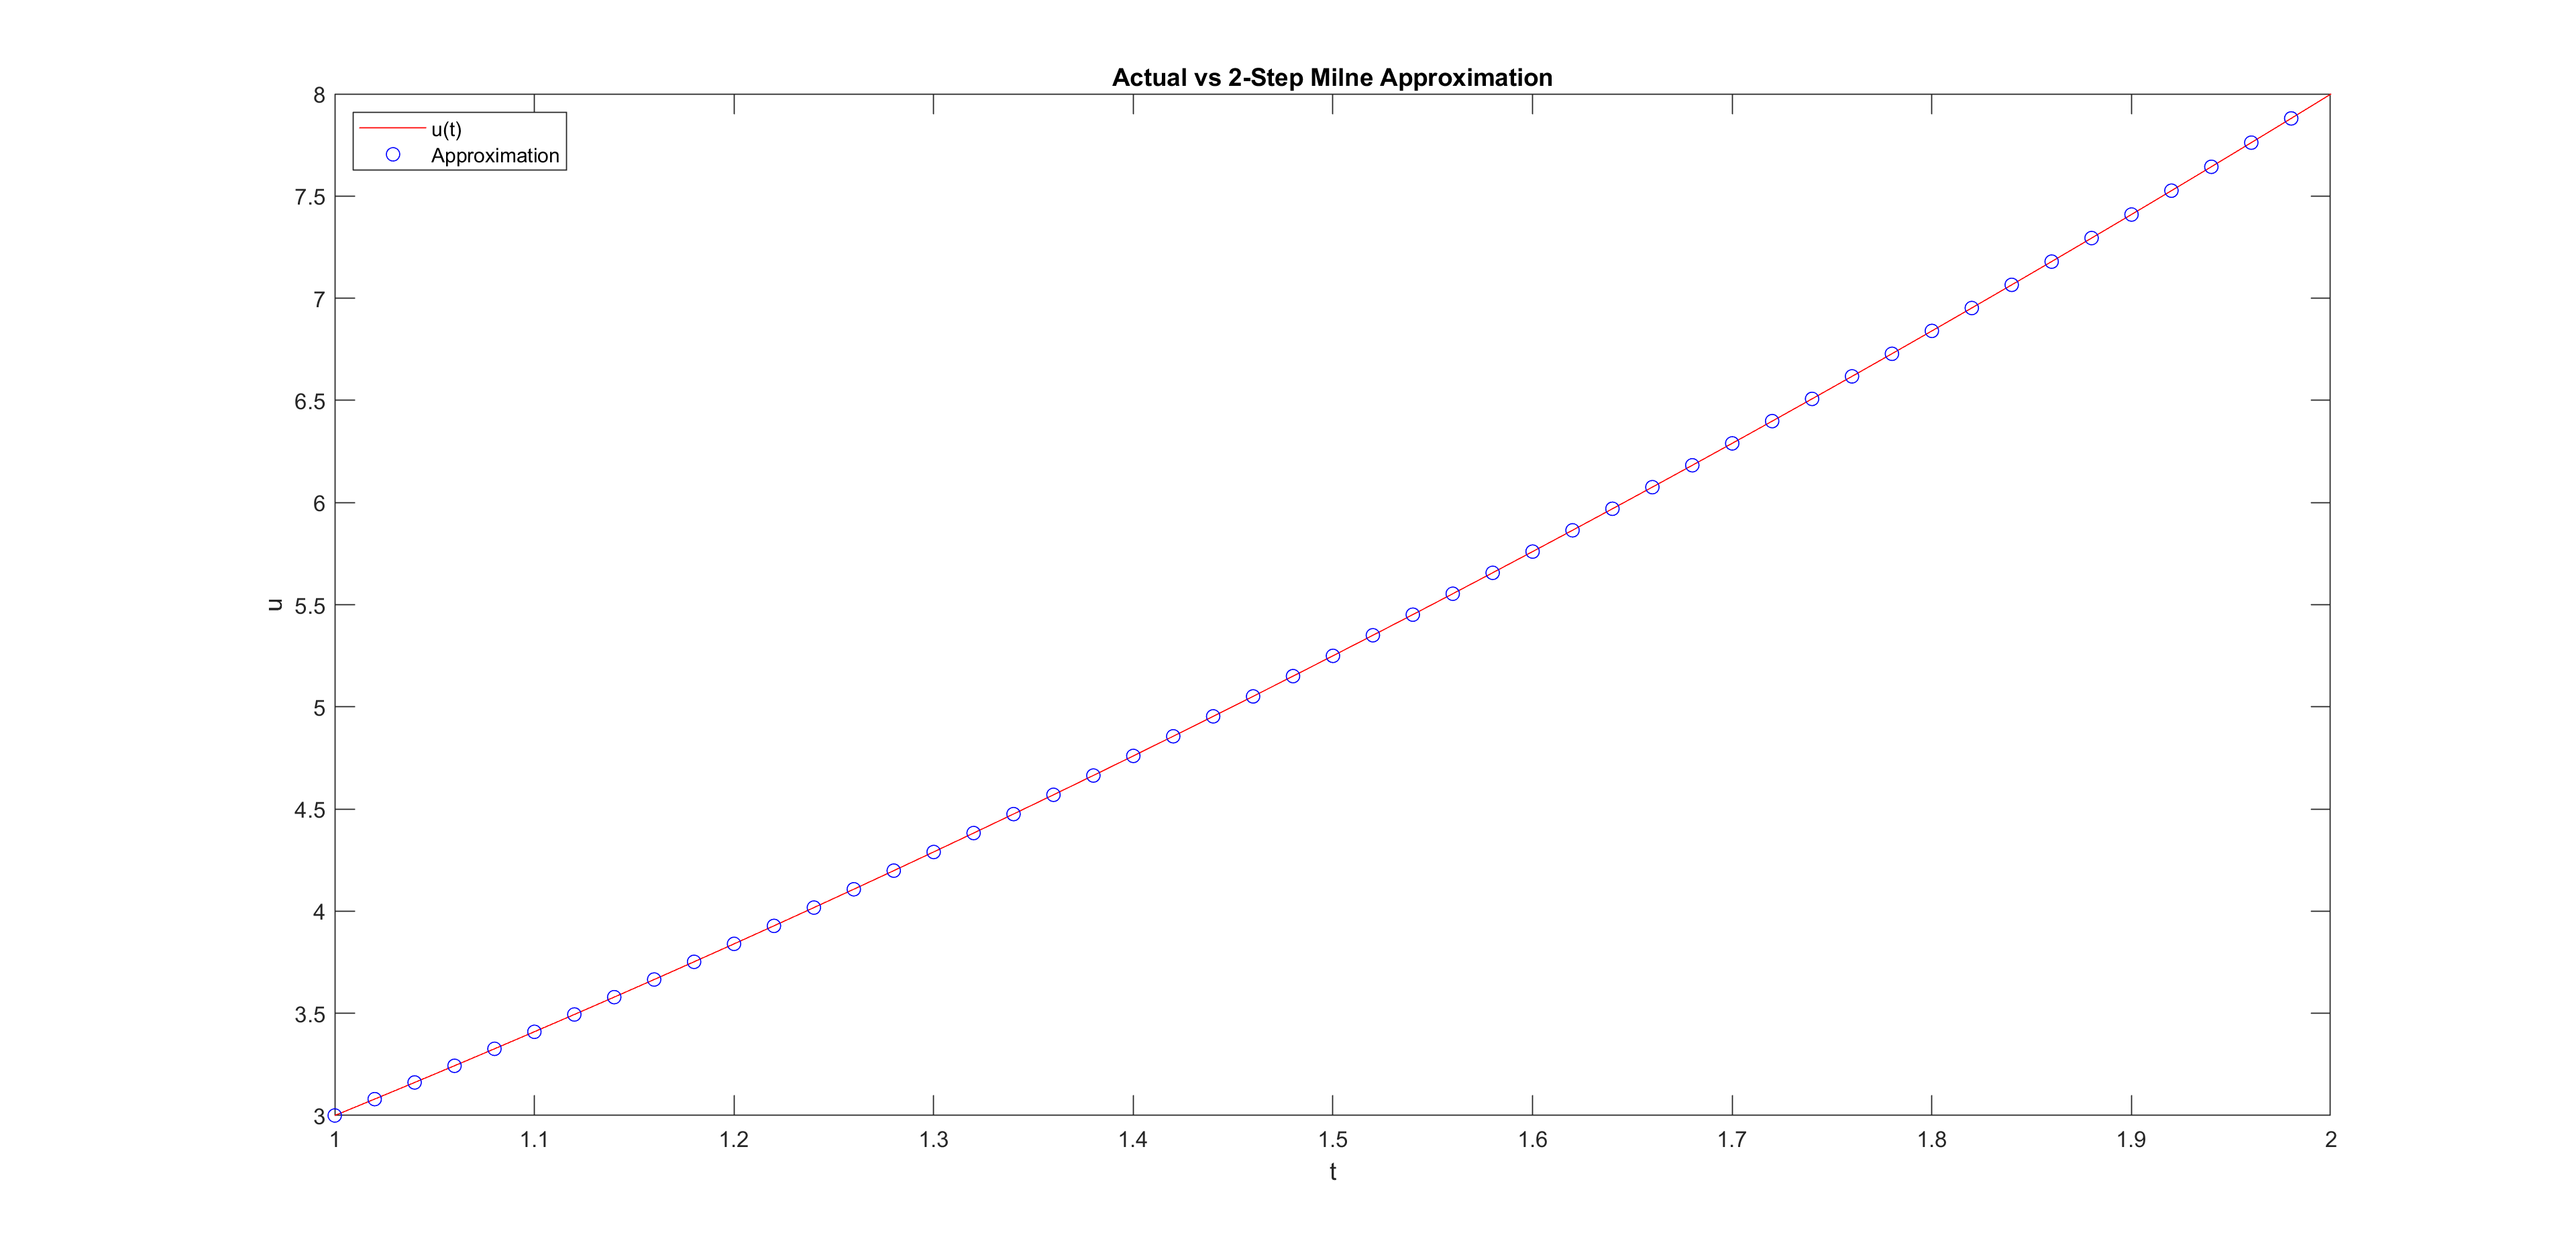
\includegraphics[scale=0.15]{2.PNG}
    \end{center}

\end{solution}

\newpage
\lstinputlisting{num2.m}